% This document is part of the transientdict project.
% Copyright 2013 the authors.

\documentclass[12pt]{article}

\newcommand{\project}[1]{\textsl{#1}}
\newcommand{\Fermi}{\project{Fermi}}
\newcommand{\RXTE}{\project{RXTE}}
\newcommand{\given}{\,|\,}
\newcommand{\dd}{\mathrm{d}}
\renewcommand{\count}{y}
\newcommand{\pars}{\theta}
\newcommand{\mean}{\lambda}
\newcommand{\Poisson}{{\mathcal P}}
\newcommand{\Uniform}{{\mathcal U}}
\newcommand{\bg}{\mathrm{bg}}
\newcommand{\word}{\phi}

\begin{document}

\section*{A model for magnetar bursts}

\noindent
Huppenkothen, Murray, Hogg, Brewer, Frean \\
\textsl{2013 December}

\paragraph{abstract}
Magnetars are whatever and people need whatever.
Magnetars produce bursts,
  each of which appears to be composed of a set of one or more spikes.
Here we build a probabilistic generative model for the \Fermi\ GBM photon data on Magnetar bursts.
The spikes appear to be somewhat asymmetric
  (rise looks different from decay),
  have various amplitudes,
  but have widths that appear to be similar \emph{within} each burst.
We model each burst as being composed of a mixture of spikes,
  where each spike is a scaled, stretched, and shifted version of a universal dimensionless function.
We perform probabilistic inference with a Poisson likelihood and vague priors to determine
  the positions, amplitudes, and positions of the spikes,
  the width of the spikes in each burst,
  and the shape of the dimensionless spike function.
The phenomenology of spike multiplicity, shape, and width is discussed.

\section{introduction}

Magnetars make bursts.
Magnetar bursts have many spikes each.
The spikes look similar within each burst.
That motivates a very simple model,
  in which each burst is made up of a sum of spike models, which we call words.

\section{data}

The ``raw'' data, for our purposes, are photon arrival times.
For magnetar SGR J1550-5418, these come from triggered photon streams telemetered down from the \Fermi\ Gamma-ray Burst Monitor (GBM).
\Fermi\/GBM is not a pointed instrument, but has twelve detectors observing the entire unocculted sky all the time. When a burst triggers the
instrument (by increased count rate), GBM will link down data streams at the native time resolution of the instrument, $2\mu\mathrm{s}$ from 
$30$ seconds before the trigger to $300$ seconds after the trigger, after which it cannot trigger for another $300$ seconds. 
Because bursts may appear within $300$s of each other, one observation (equivalent to one trigger of length $330$s) may include more than one
bursts, and one must find the untriggered bursts in the data.

The data streams are affected by dead time and saturation. Saturation cuts off the number of recorded photons at the maximum rate
that the science data bus on board the spacecraft can transmit, $3.5 \times 10^{5} \, \mathrm{counts}/\mathrm{s}$ per detector. This means
that exceptionally bright bursts will flatten out above that count rate. We exclude any bursts with count rates $>3.5\times10^{5} \, \mathrm{cts}/\mathrm{s}$.
Dead time occurs because the instrument cannot record a second photon within $2.6\mu\mathrm{s}$ of arrival of a previous photon. 
The second photon is thus either not recorded at all, or, on occasion, recorded as a single photon with the combined energy. This effectively 
imposes a time scale onto the data, which means that the data then deviate away from the expected Poisson distribution. 
Dead time is harder to quantify and account for than saturation. It is possible to correct count rates based on simulations of the instrument (REF, Bhat et al, 2013),
but this will not correct the statistical distributions. We currently don't take dead time into account in our analysis. 

We currently use light curves with a time resolution of $0.1\,\mathrm{ms}$. The time resolution is chosen small enough to preserve features
in the data on short time scales, while at the same time have a reasonable number of counts per time bin. 
Burst durations are defined in $T90$, the time in which $90\%$ of photons arrive at the detector, with $0.2T90$ added on either side
to make sure the entire burst is included. 

Data for the strongest-field magnetars SGR 1806-20 and SGR 1900+14 are recorded with the {\it Rossi} X-ray Timing Explorer (\RXTE), which someone
else will write the details about (but data are still time-tagged photon events and suffer from saturation and dead time). 

%There are many small details.
%We choose [what binning and why?].
%We use data [in what interval?] around each burst.

In what follows, the data for one burst are photon counts $\count_n$ (integer) in $N$ bins $n$.
The data from a few example bursts are shown in Figure \ref{fig:example_bursts}.

%\begin{figure*}[h]
%\begin{center}
%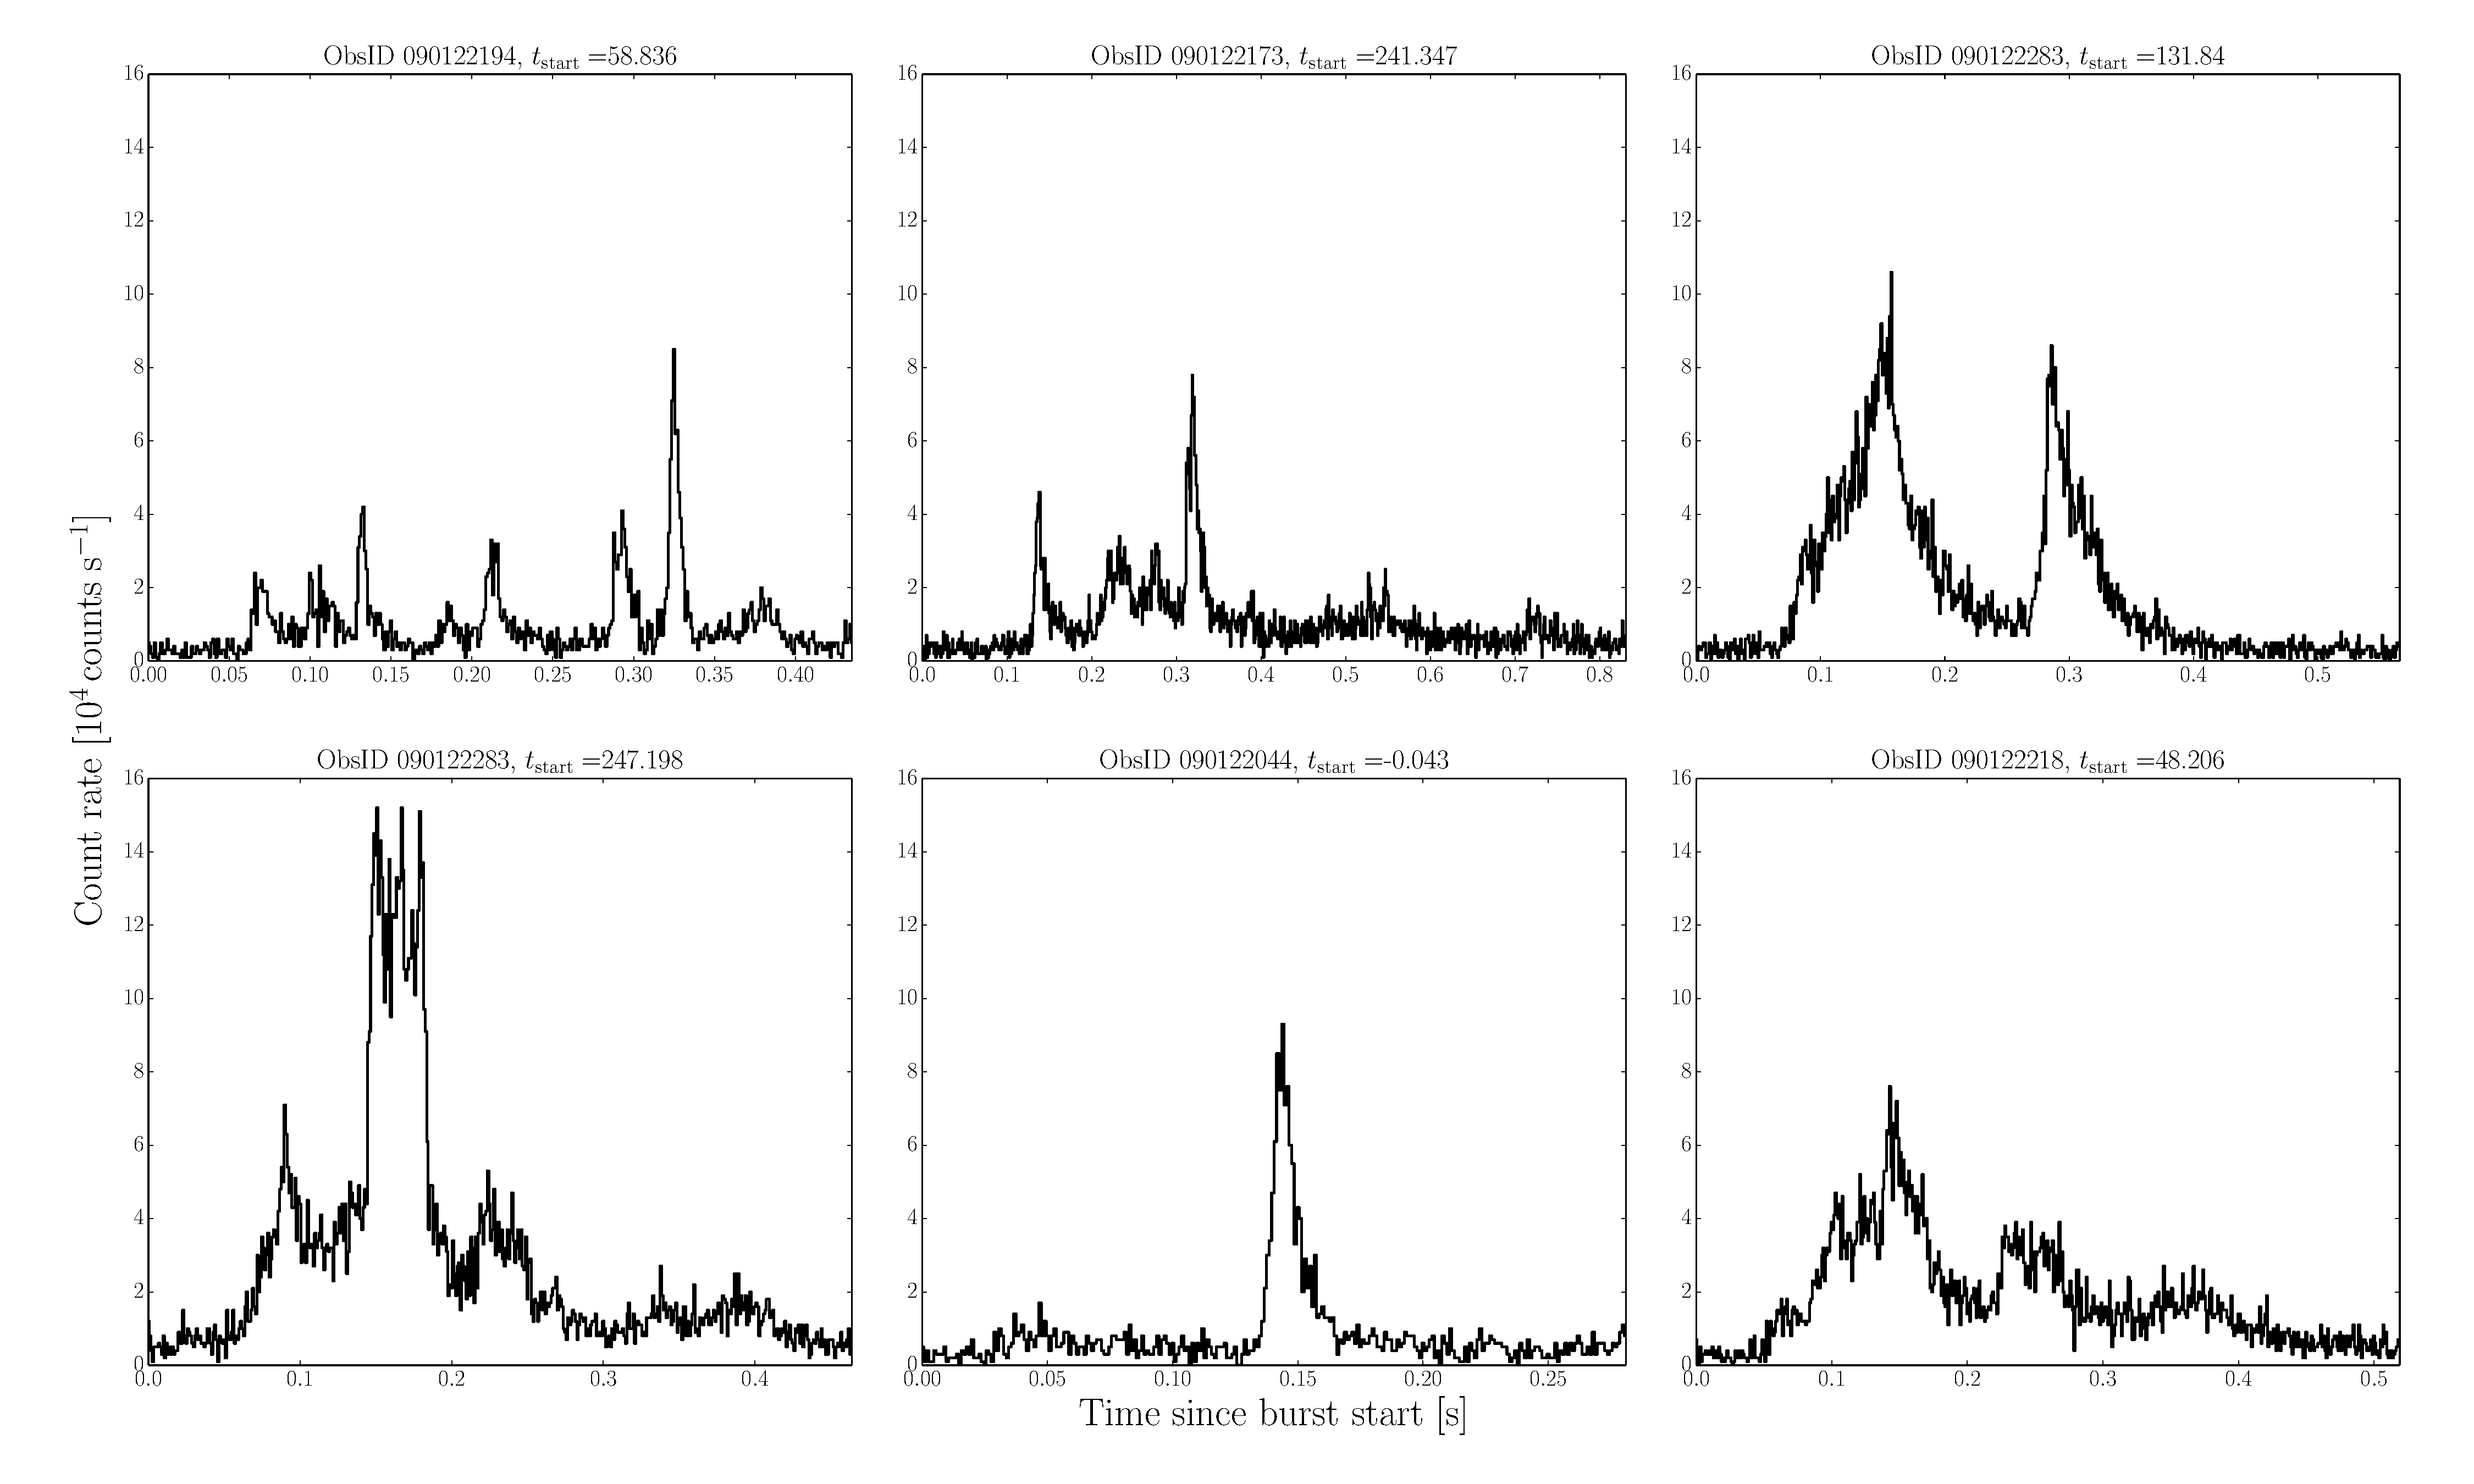
\includegraphics[width=18cm]{example_bursts.png}
%\caption{}
%\label{fig:example_bursts}
%\end{center}
%\end{figure*}



\section{model}

The model for the data in or near one burst is
\begin{eqnarray}
p(\count_n\given\pars) &=& \Poisson(\count_n\given\mean_n)
\\
\mean_n &=& \mean_{\bg} + \sum_{k=1}^K \mean_{nk}
\\
\mean_{nk} &\equiv& \int_{t_n-\Delta/2}^{t_n+\Delta/2} A_k\,\word(\frac{t'-t_k}{\tau})\,\dd t'
\\
\word(\xi) &=& \left\{\begin{array}{ll}\exp(\xi) & \mbox{for $\xi<0$}\\ \exp(-\xi/s) & \mbox{for $\xi\geq 0$}\end{array}\right. \, ,
\end{eqnarray}

where $\Poisson(\count\given\mean)$ is the Poisson probability of getting count $y$ given mean rate $\mean$,
  $\pars$ is the vector or blob of all model parameters,
  $\mean_{\bg}$ is the background (DC) level in the bin,
  $t_n$ is the time of the center of the bin,
  $\Delta$ is the full width of the bin,
  $K$ is the number of words (spikes) $k$ making up the burst,
  $\phi(\xi)$ is the dimensionless word function,
  $A_k, t_k$ are the amplitudes and time offsets of the words,
  and $s, \tau$ set the shape (asymmetry or skew) and rise time of the words.
  
Various parameters can be left free completely, or can be tied together between words:
 
\begin{equation}
\theta \equiv [,\{t_k, \tau_k, A_k, s_k \}_{k=1}^K, \mean_{\bg} ]
\end{equation}

for complete freedom of word parameters between words,

\begin{equation}
\theta \equiv [,\{t_k, A_k, s_k \}_{k=1}^K,  \tau_k, \mean_{\bg} ]
\end{equation}

for tying the rise time together within a burst, and

\begin{equation}
\theta \equiv [,\{t_k, A_k\}_{k=1}^K, \tau_k, s_k , \mean_{\bg} ]\end{equation}

for a model where both the rise time and the skewness are tied together for all words within a burst.

%\begin{figure*}[h]
%\begin{center}
%\includegraphics[width=18cm]{example_words.png}
%\caption{}
%\label{fig:example_words}
%\end{center}
%\end{figure*}

  
Figure \ref{fig:example_words} shows the shape of a word
  and an example of a burst generated by our model.

The model for a large set of bursts is whatever.
[We should probably, in the above, index bursts $m$,
  and maybe even magnetar $j$.]

\emph{Notes to selves:}
At one point we figured we could \emph{fix} shape parameter $s$
  to be the same for all the words in all the bursts from one magnetar,
  but permit the duration $\tau$ to vary.
However, as we worked in our coding session we moved more in the direction
  of thinking in terms of ``rise time'' $\tau$ and decay time $s\,\tau$.
It might be better to parameterize that way.
One possible point of discovery would be that the rise times
  are fundamental to each magnetar,
  but decay times vary.
(For instance.)

The prior pdfs are
\begin{eqnarray}
p(\ln\lambda_{\bg}) &=& \Uniform(\ln\lambda_{\bg}\given a_1, a_2)
\\
p(\ln s) &=& \Uniform(\ln s\given a_3, a_4)
\\
p(\ln\tau) &=& \Uniform(\ln\tau\given a_5, a_6)
\\
p(\ln A_k) &=& \Uniform(\ln A_k\given a_7, a_8)
\\
p(t_k) &=& \Uniform(t_k\given a_9, a_{10})
\quad,
\end{eqnarray}
where $\Uniform(x\given a, b)$ is the uniform distribution for $x$ in the range $a<x<b$.

We use \project{emcee} (CITE) to perform MCMC sampling.
[We initialize the MCMC walkers how?]

Finally, there is the issue of how to set the number $K$ of words in each burst.
We take a ``cross-validation'' approach [take that, BJB],
  in which we ask what value of $K$ does the best job at making posterior predictions
  about left-out data.
[We construct this validation test how?]
Figure [what figure?] shows an example burst,
  fit with $K=1$, $2$, $3$, $4$, and $5$ words.
It also shows the result of the posterior-prediction validation
  that selects $K=4$ as the best choice for this burst.

\section{results}

\section{discussion}

\paragraph{acknowledgements}
We thank the organizers of MaxEnt2013.

\end{document}
